\documentclass[aspectratio=169,12pt]{beamer}

% Theme and colors
\usetheme{Madrid}
\usecolortheme{whale}
\setbeamertemplate{navigation symbols}{}
\setbeamertemplate{footline}[frame number]

% Packages
\usepackage{amsmath,amssymb,amsthm}
\usepackage{graphicx}
\usepackage{tikz}
\usetikzlibrary{trees,shapes,arrows,positioning,calc}
\usepackage{booktabs}
\usepackage{array}
\usepackage{multirow}
\usepackage{algorithm}
\usepackage{algorithmic}
\usepackage{xcolor}
\usepackage{hyperref}

% Custom colors
\definecolor{codegreen}{rgb}{0,0.6,0}
\definecolor{codepurple}{rgb}{0.58,0,0.82}
\definecolor{darkblue}{rgb}{0,0,0.7}

% Title information
\title[Huffman Coding]{Huffman Coding}
\subtitle{Optimal Prefix-Free Data Compression}
\author[Mahesh C]{\textbf{Mahesh C}\\FISAT}
\institute{Federal Institute of Science and Technology (FISAT)\\Multimedia Technology Class}
\date{\today}

\begin{document}

% Title slide
\begin{frame}
    \titlepage
\end{frame}

% Outline
\begin{frame}{Outline}
    \tableofcontents
\end{frame}

%==============================================================================
\section{Quick Recap: Why Variable-Length Codes?}
%==============================================================================

\begin{frame}{Remember Shannon-Fano?}
    \begin{columns}
        \begin{column}{0.5\textwidth}
            \textbf{Key Ideas from Last Class:}
            \begin{itemize}
                \item Frequent symbols $\rightarrow$ Short codes
                \item Rare symbols $\rightarrow$ Long codes
                \item Prefix-free for instant decoding
                \item Top-down divide approach
            \end{itemize}
            
            \vspace{0.3cm}
            \textbf{Shannon-Fano Limitation:}
            \begin{itemize}
                \item Not always optimal
                \item Division may not be perfect
                \item Can we do better?
            \end{itemize}
        \end{column}
        \begin{column}{0.5\textwidth}
            \begin{block}{The Question}
                Is there a method that \textbf{always} produces the optimal prefix-free code?
            \end{block}
            
            \vspace{0.5cm}
            \begin{alertblock}{Answer: YES!}
                \textbf{Huffman Coding} (1952)
                
                Guaranteed optimal for symbol-by-symbol coding!
            \end{alertblock}
        \end{column}
    \end{columns}
\end{frame}

\begin{frame}{A Simple Puzzle to Start}
    \begin{center}
        \Large{\textbf{You have 4 items with weights: 1, 2, 3, 4}}
        
        \vspace{0.5cm}
        \textit{How would you pair them to minimize total ``cost''?}
    \end{center}
    
    \vspace{0.5cm}
    \begin{columns}
        \begin{column}{0.5\textwidth}
            \textbf{Option A:} Pair heaviest first
            \begin{itemize}
                \item (4+3) = 7, then (7+2) = 9, then (9+1) = 10
            \end{itemize}
        \end{column}
        \begin{column}{0.5\textwidth}
            \textbf{Option B:} Pair lightest first
            \begin{itemize}
                \item (1+2) = 3, then (3+3) = 6, then (6+4) = 10
            \end{itemize}
        \end{column}
    \end{columns}
    
    \vspace{0.5cm}
    \pause
    \begin{block}{Huffman's Insight}
        Always combine the \textbf{two smallest} items first!
        
        This greedy approach leads to optimal results.
    \end{block}
\end{frame}

%==============================================================================
\section{Introduction to Huffman Coding}
%==============================================================================

\begin{frame}{Who is David Huffman?}
    \begin{columns}
        \begin{column}{0.6\textwidth}
            \textbf{The Story (1951):}
            \begin{itemize}
                \item MIT graduate student
                \item Professor Robert Fano's class
                \item Term paper OR final exam choice
                \item Paper topic: Find optimal binary codes
            \end{itemize}
            
            \vspace{0.3cm}
            \textbf{The Breakthrough:}
            \begin{itemize}
                \item Huffman almost gave up
                \item Threw away his notes in frustration
                \item Suddenly realized: \textbf{build bottom-up!}
                \item Proved it was optimal
            \end{itemize}
        \end{column}
        \begin{column}{0.4\textwidth}
            \begin{block}{Fun Fact}
                Huffman's algorithm beat his professor's own Shannon-Fano method!
                
                \vspace{0.3cm}
                Published in 1952, still used today in:
                \begin{itemize}
                    \item JPEG images
                    \item MP3 audio
                    \item ZIP files
                    \item DEFLATE
                \end{itemize}
            \end{block}
        \end{column}
    \end{columns}
\end{frame}

\begin{frame}{What is Huffman Coding?}
    \begin{block}{Definition}
        Huffman coding is a \textbf{greedy algorithm} that constructs an \textbf{optimal prefix-free} binary code by building a tree from the \textbf{bottom up}.
    \end{block}
    
    \vspace{0.3cm}
    \textbf{Key Properties:}
    \begin{itemize}
        \item \textcolor{codegreen}{Optimal} --- Minimum average code length among all prefix codes
        \item \textcolor{darkblue}{Prefix-free} --- No codeword is a prefix of another
        \item \textcolor{codepurple}{Bottom-up} --- Start with leaves, build toward root
        \item \textbf{Greedy} --- Always merge two smallest probability nodes
    \end{itemize}
    
    \vspace{0.3cm}
    \begin{alertblock}{Key Difference from Shannon-Fano}
        \begin{center}
            Shannon-Fano: \textbf{Top-down} (divide) \hspace{1cm} Huffman: \textbf{Bottom-up} (merge)
        \end{center}
    \end{alertblock}
\end{frame}

\begin{frame}{The Core Idea: Build a Tree}
    \begin{center}
        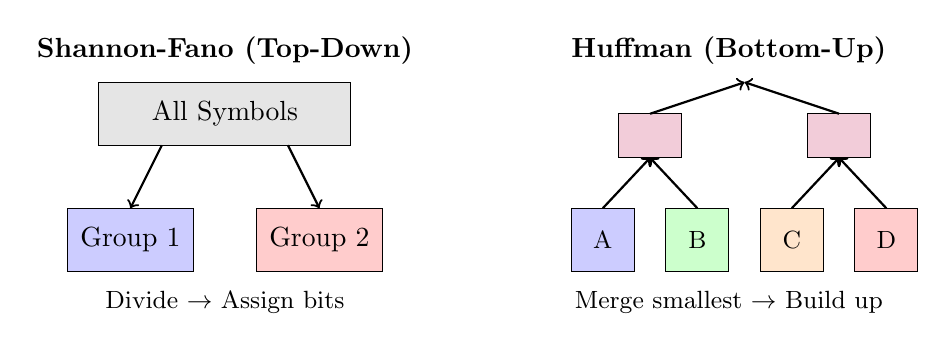
\begin{tikzpicture}[scale=0.8]
            % Shannon-Fano approach
            \node at (-4,3.5) {\textbf{Shannon-Fano (Top-Down)}};
            \draw[fill=gray!20] (-6,2) rectangle (-2,3);
            \node at (-4,2.5) {All Symbols};
            \draw[->,thick] (-5,2) -- (-5.5,1);
            \draw[->,thick] (-3,2) -- (-2.5,1);
            \draw[fill=blue!20] (-6.5,0) rectangle (-4.5,1);
            \draw[fill=red!20] (-3.5,0) rectangle (-1.5,1);
            \node at (-5.5,0.5) {Group 1};
            \node at (-2.5,0.5) {Group 2};
            \node at (-4,-0.5) {\small Divide $\rightarrow$ Assign bits};
            
            % Huffman approach
            \node at (4,3.5) {\textbf{Huffman (Bottom-Up)}};
            \draw[fill=blue!20] (1.5,0) rectangle (2.5,1);
            \draw[fill=green!20] (3,0) rectangle (4,1);
            \draw[fill=orange!20] (4.5,0) rectangle (5.5,1);
            \draw[fill=red!20] (6,0) rectangle (7,1);
            \node at (2,0.5) {\small A};
            \node at (3.5,0.5) {\small B};
            \node at (5,0.5) {\small C};
            \node at (6.5,0.5) {\small D};
            \draw[->,thick] (2,1) -- (2.75,1.8);
            \draw[->,thick] (3.5,1) -- (2.75,1.8);
            \draw[fill=purple!20] (2.25,1.8) rectangle (3.25,2.5);
            \draw[->,thick] (2.75,2.5) -- (4.25,3);
            \draw[->,thick] (5,1) -- (5.75,1.8);
            \draw[->,thick] (6.5,1) -- (5.75,1.8);
            \draw[fill=purple!20] (5.25,1.8) rectangle (6.25,2.5);
            \draw[->,thick] (5.75,2.5) -- (4.25,3);
            \node at (4,-0.5) {\small Merge smallest $\rightarrow$ Build up};
        \end{tikzpicture}
    \end{center}

\end{frame}

%==============================================================================
\section{Huffman Algorithm}
%==============================================================================

\begin{frame}{The Huffman Algorithm}
    \begin{block}{Algorithm Steps}
        \begin{enumerate}
            \item Create a \textbf{leaf node} for each symbol with its probability
            \item Put all nodes in a \textbf{priority queue} (min-heap by probability)
            \item While more than one node remains:
            \begin{enumerate}
                \item Remove the \textbf{two nodes} with lowest probability
                \item Create a \textbf{new internal node} with these as children
                \item New node's probability = sum of children's probabilities
                \item Add new node back to the queue
            \end{enumerate}
            \item The remaining node is the \textbf{root} of the Huffman tree
            \item Assign \textbf{0} to left branches, \textbf{1} to right branches
        \end{enumerate}
    \end{block}
\end{frame}

\begin{frame}{Algorithm Pseudocode}
    \begin{algorithm}[H]
        \caption{Huffman Coding}
        \begin{algorithmic}[1]
            \STATE \textbf{Input:} Symbols $S = \{s_1, s_2, \ldots, s_n\}$ with probabilities $P$
            \STATE \textbf{Output:} Huffman tree (optimal prefix-free code)
            \STATE
            \STATE Create leaf node for each symbol
            \STATE $Q \leftarrow$ priority queue of all nodes (by probability)
            \WHILE{$|Q| > 1$}
                \STATE $left \leftarrow$ ExtractMin($Q$)
                \STATE $right \leftarrow$ ExtractMin($Q$)
                \STATE Create new node $z$ with children $left$, $right$
                \STATE $z.prob \leftarrow left.prob + right.prob$
                \STATE Insert($Q$, $z$)
            \ENDWHILE
            \STATE \textbf{return} ExtractMin($Q$) \COMMENT{Root of Huffman tree}
        \end{algorithmic}
    \end{algorithm}
\end{frame}

\begin{frame}{Why Does This Work?}
    \textbf{Greedy Choice Property:}
    
    \begin{block}{Lemma 1}
        The two symbols with the \textbf{lowest probabilities} must have the \textbf{longest codes} in any optimal code.
    \end{block}
    
    \begin{block}{Lemma 2}
        The two symbols with lowest probabilities can be made \textbf{siblings} (same parent) in an optimal tree without increasing average code length.
    \end{block}
    
    \vspace{0.3cm}
    \textbf{Intuition:}
    \begin{itemize}
        \item Rare symbols should be deep in the tree (long codes)
        \item Merging them first puts them at the bottom
        \item Their combined probability competes with others
        \item Process continues optimally
    \end{itemize}
\end{frame}

%==============================================================================
\section{Step-by-Step Example}
%==============================================================================

\begin{frame}{Example: Building a Huffman Tree}
    \textbf{Given:} Source symbols with probabilities:
    
    \begin{center}
        \begin{tabular}{c|ccccc}
            \toprule
            Symbol & A & B & C & D & E \\
            \midrule
            Probability & 0.35 & 0.25 & 0.20 & 0.12 & 0.08 \\
            \bottomrule
        \end{tabular}
    \end{center}
    
    \vspace{0.5cm}
    \textbf{Step 1:} Create leaf nodes and put in priority queue
    
    \begin{center}
        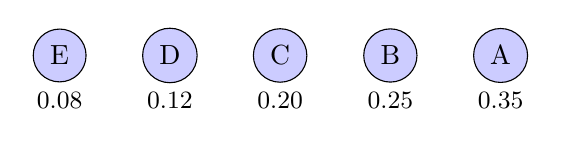
\begin{tikzpicture}[scale=0.7]
            \node[draw, circle, fill=blue!20] (E) at (0,0) {E};
            \node[below] at (0,-0.5) {\small 0.08};
            
            \node[draw, circle, fill=blue!20] (D) at (2,0) {D};
            \node[below] at (2,-0.5) {\small 0.12};
            
            \node[draw, circle, fill=blue!20] (C) at (4,0) {C};
            \node[below] at (4,-0.5) {\small 0.20};
            
            \node[draw, circle, fill=blue!20] (B) at (6,0) {B};
            \node[below] at (6,-0.5) {\small 0.25};
            
            \node[draw, circle, fill=blue!20] (A) at (8,0) {A};
            \node[below] at (8,-0.5) {\small 0.35};
        \end{tikzpicture}
    \end{center}
    
    \textit{Queue (sorted): E(0.08), D(0.12), C(0.20), B(0.25), A(0.35)}
\end{frame}

\begin{frame}{Example: Step 2 --- First Merge}
    \textbf{Merge two smallest:} E(0.08) + D(0.12) = 0.20
    
    \begin{center}
        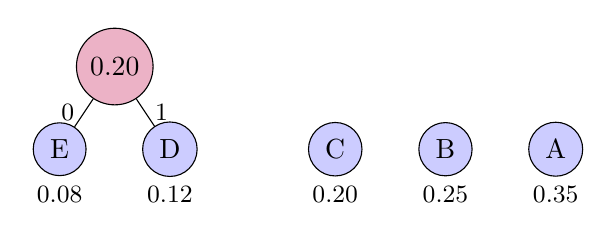
\begin{tikzpicture}[scale=0.7]
            % Merged node
            \node[draw, circle, fill=purple!30] (ED) at (1,1.5) {0.20};
            \node[draw, circle, fill=blue!20] (E) at (0,0) {E};
            \node[draw, circle, fill=blue!20] (D) at (2,0) {D};
            \draw (ED) -- (E) node[midway, left] {\small 0};
            \draw (ED) -- (D) node[midway, right] {\small 1};
            \node[below] at (0,-0.5) {\small 0.08};
            \node[below] at (2,-0.5) {\small 0.12};
            
            % Remaining nodes
            \node[draw, circle, fill=blue!20] (C) at (5,0) {C};
            \node[below] at (5,-0.5) {\small 0.20};
            
            \node[draw, circle, fill=blue!20] (B) at (7,0) {B};
            \node[below] at (7,-0.5) {\small 0.25};
            
            \node[draw, circle, fill=blue!20] (A) at (9,0) {A};
            \node[below] at (9,-0.5) {\small 0.35};
        \end{tikzpicture}
    \end{center}
    
    \vspace{0.3cm}
    \textit{Queue (sorted): C(0.20), [ED](0.20), B(0.25), A(0.35)}
    
    \vspace{0.2cm}
    \textbf{Note:} When probabilities are equal, either order works!
\end{frame}

\begin{frame}{Example: Step 3 --- Second Merge}
    \textbf{Merge two smallest:} C(0.20) + [ED](0.20) = 0.40
    
    \begin{center}
        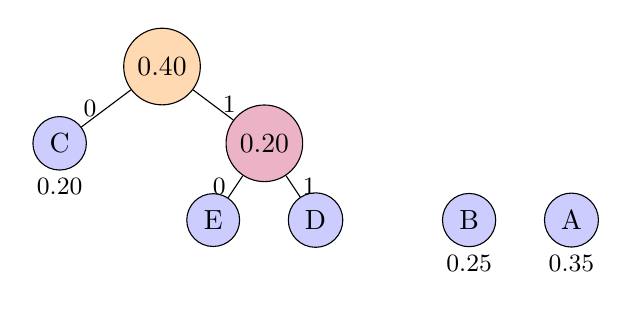
\begin{tikzpicture}[scale=0.65]
            % Top merged node
            \node[draw, circle, fill=orange!30] (CED) at (2,3) {0.40};
            
            % C branch
            \node[draw, circle, fill=blue!20] (C) at (0,1.5) {C};
            \draw (CED) -- (C) node[midway, left] {\small 0};
            \node[below] at (0,1) {\small 0.20};
            
            % ED branch
            \node[draw, circle, fill=purple!30] (ED) at (4,1.5) {0.20};
            \draw (CED) -- (ED) node[midway, right] {\small 1};
            
            \node[draw, circle, fill=blue!20] (E) at (3,0) {E};
            \node[draw, circle, fill=blue!20] (D) at (5,0) {D};
            \draw (ED) -- (E) node[midway, left] {\small 0};
            \draw (ED) -- (D) node[midway, right] {\small 1};
            
            % Remaining nodes
            \node[draw, circle, fill=blue!20] (B) at (8,0) {B};
            \node[below] at (8,-0.5) {\small 0.25};
            
            \node[draw, circle, fill=blue!20] (A) at (10,0) {A};
            \node[below] at (10,-0.5) {\small 0.35};
        \end{tikzpicture}
    \end{center}
    
    \vspace{0.3cm}
    \textit{Queue (sorted): B(0.25), A(0.35), [CED](0.40)}
\end{frame}

\begin{frame}{Example: Step 4 --- Third Merge}
    \textbf{Merge two smallest:} B(0.25) + A(0.35) = 0.60
    
    \begin{center}
        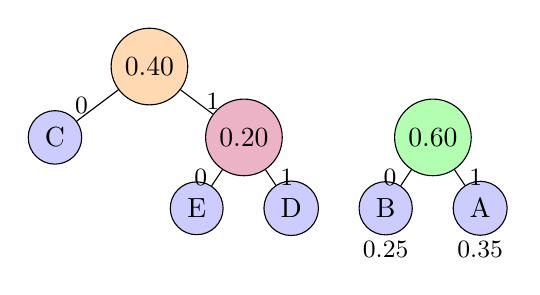
\begin{tikzpicture}[scale=0.6]
            % BA merged
            \node[draw, circle, fill=green!30] (BA) at (8,1.5) {0.60};
            \node[draw, circle, fill=blue!20] (B) at (7,0) {B};
            \node[draw, circle, fill=blue!20] (A) at (9,0) {A};
            \draw (BA) -- (B) node[midway, left] {\small 0};
            \draw (BA) -- (A) node[midway, right] {\small 1};
            \node[below] at (7,-0.5) {\small 0.25};
            \node[below] at (9,-0.5) {\small 0.35};
            
            % CED tree
            \node[draw, circle, fill=orange!30] (CED) at (2,3) {0.40};
            \node[draw, circle, fill=blue!20] (C) at (0,1.5) {C};
            \draw (CED) -- (C) node[midway, left] {\small 0};
            
            \node[draw, circle, fill=purple!30] (ED) at (4,1.5) {0.20};
            \draw (CED) -- (ED) node[midway, right] {\small 1};
            
            \node[draw, circle, fill=blue!20] (E) at (3,0) {E};
            \node[draw, circle, fill=blue!20] (D) at (5,0) {D};
            \draw (ED) -- (E) node[midway, left] {\small 0};
            \draw (ED) -- (D) node[midway, right] {\small 1};
        \end{tikzpicture}
    \end{center}
    
    \vspace{0.3cm}
    \textit{Queue (sorted): [CED](0.40), [BA](0.60)}
\end{frame}

\begin{frame}{Example: Step 5 --- Final Merge (Root)}
    \textbf{Merge last two:} [CED](0.40) + [BA](0.60) = 1.00
    
    \begin{center}
        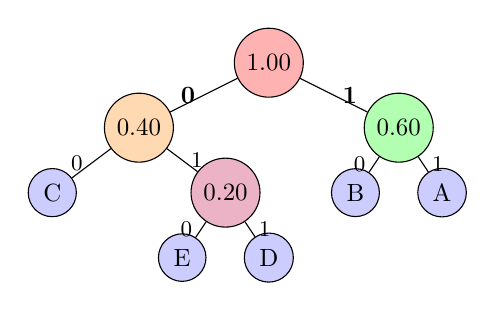
\begin{tikzpicture}[scale=0.55, every node/.style={scale=0.9}]
            % Root
            \node[draw, circle, fill=red!30] (Root) at (5,5) {1.00};
            
            % Left subtree (CED)
            \node[draw, circle, fill=orange!30] (CED) at (2,3.5) {0.40};
            \draw (Root) -- (CED) node[midway, left] {\textbf{0}};
            
            \node[draw, circle, fill=blue!20] (C) at (0,2) {C};
            \draw (CED) -- (C) node[midway, left] {\small 0};
            
            \node[draw, circle, fill=purple!30] (ED) at (4,2) {0.20};
            \draw (CED) -- (ED) node[midway, right] {\small 1};
            
            \node[draw, circle, fill=blue!20] (E) at (3,0.5) {E};
            \node[draw, circle, fill=blue!20] (D) at (5,0.5) {D};
            \draw (ED) -- (E) node[midway, left] {\small 0};
            \draw (ED) -- (D) node[midway, right] {\small 1};
            
            % Right subtree (BA)
            \node[draw, circle, fill=green!30] (BA) at (8,3.5) {0.60};
            \draw (Root) -- (BA) node[midway, right] {\textbf{1}};
            
            \node[draw, circle, fill=blue!20] (B) at (7,2) {B};
            \node[draw, circle, fill=blue!20] (A) at (9,2) {A};
            \draw (BA) -- (B) node[midway, left] {\small 0};
            \draw (BA) -- (A) node[midway, right] {\small 1};
        \end{tikzpicture}
    \end{center}
    
    \vspace{0.2cm}
    \textbf{Huffman Tree Complete!}
\end{frame}

\begin{frame}{Example: Reading the Codes}
    \textbf{Traverse from root to each leaf, collecting 0s and 1s:}
    
    \begin{columns}
        \begin{column}{0.5\textwidth}
            \begin{center}
                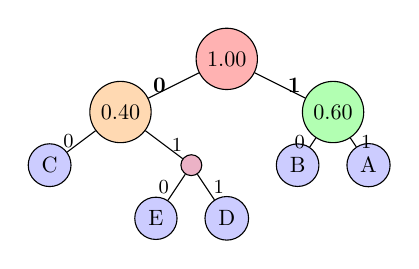
\begin{tikzpicture}[scale=0.45, every node/.style={scale=0.8}]
                    \node[draw, circle, fill=red!30] (Root) at (5,5) {1.00};
                    \node[draw, circle, fill=orange!30] (CED) at (2,3.5) {0.40};
                    \draw (Root) -- (CED) node[midway, left] {\textbf{0}};
                    \node[draw, circle, fill=blue!20] (C) at (0,2) {C};
                    \draw (CED) -- (C) node[midway, left] {\small 0};
                    \node[draw, circle, fill=purple!30] (ED) at (4,2) {};
                    \draw (CED) -- (ED) node[midway, right] {\small 1};
                    \node[draw, circle, fill=blue!20] (E) at (3,0.5) {E};
                    \node[draw, circle, fill=blue!20] (D) at (5,0.5) {D};
                    \draw (ED) -- (E) node[midway, left] {\small 0};
                    \draw (ED) -- (D) node[midway, right] {\small 1};
                    \node[draw, circle, fill=green!30] (BA) at (8,3.5) {0.60};
                    \draw (Root) -- (BA) node[midway, right] {\textbf{1}};
                    \node[draw, circle, fill=blue!20] (B) at (7,2) {B};
                    \node[draw, circle, fill=blue!20] (A) at (9,2) {A};
                    \draw (BA) -- (B) node[midway, left] {\small 0};
                    \draw (BA) -- (A) node[midway, right] {\small 1};
                \end{tikzpicture}
            \end{center}
        \end{column}
        \begin{column}{0.5\textwidth}
            \textbf{Final Huffman Codes:}
            \begin{center}
                \begin{tabular}{c|c|c|c}
                    \toprule
                    Symbol & Prob & Code & Len \\
                    \midrule
                    A & 0.35 & 11 & 2 \\
                    B & 0.25 & 10 & 2 \\
                    C & 0.20 & 00 & 2 \\
                    D & 0.12 & 011 & 3 \\
                    E & 0.08 & 010 & 3 \\
                    \bottomrule
                \end{tabular}
            \end{center}
            
            \vspace{0.3cm}
            \textbf{Verify prefix-free:}
            
            No code is prefix of another \checkmark
        \end{column}
    \end{columns}
\end{frame}

%==============================================================================
\section{Performance Analysis}
%==============================================================================

\begin{frame}{Average Code Length Calculation}
    \begin{block}{Average Code Length}
        \begin{equation}
            L_{avg} = \sum_{i=1}^{n} p_i \cdot l_i
        \end{equation}
    \end{block}
    
    \vspace{0.3cm}
    \textbf{For our Huffman code:}
    \begin{center}
        \begin{tabular}{c|c|c|c}
            \toprule
            Symbol & Probability & Code Length & $p_i \times l_i$ \\
            \midrule
            A & 0.35 & 2 & 0.70 \\
            B & 0.25 & 2 & 0.50 \\
            C & 0.20 & 2 & 0.40 \\
            D & 0.12 & 3 & 0.36 \\
            E & 0.08 & 3 & 0.24 \\
            \midrule
            \multicolumn{3}{r|}{\textbf{Total:}} & \textbf{2.20} \\
            \bottomrule
        \end{tabular}
    \end{center}
    
    $L_{avg} = \boxed{2.20 \text{ bits/symbol}}$
\end{frame}

\begin{frame}{Comparison with Entropy}
    \textbf{Entropy of the source:}
    \begin{align*}
        H(X) &= -\sum_{i} p_i \log_2 p_i \\
        &= -(0.35 \log_2 0.35 + 0.25 \log_2 0.25 + 0.20 \log_2 0.20 \\
        &\quad + 0.12 \log_2 0.12 + 0.08 \log_2 0.08) \\
        &= 0.530 + 0.500 + 0.464 + 0.367 + 0.292 \\
        &= \boxed{2.153 \text{ bits/symbol}}
    \end{align*}
    
    \vspace{0.3cm}
    \begin{block}{Efficiency}
        \begin{equation*}
            \eta = \frac{H(X)}{L_{avg}} \times 100\% = \frac{2.153}{2.20} \times 100\% = \boxed{97.86\%}
        \end{equation*}
    \end{block}
    
    \textbf{Redundancy:} $R = L_{avg} - H(X) = 2.20 - 2.153 = \boxed{0.047 \text{ bits/symbol}}$
\end{frame}

\begin{frame}{Huffman vs Shannon-Fano: Same Example}
    \textbf{Using the same probabilities:} A(0.35), B(0.25), C(0.20), D(0.12), E(0.08)
    
    \begin{columns}
        \begin{column}{0.5\textwidth}
            \textbf{Shannon-Fano Codes:}
            \begin{center}
                \begin{tabular}{c|c|c}
                    Symbol & Code & Len \\
                    \midrule
                    A & 00 & 2 \\
                    B & 01 & 2 \\
                    C & 10 & 2 \\
                    D & 110 & 3 \\
                    E & 111 & 3 \\
                \end{tabular}
            \end{center}
            $L_{avg} = 2.20$ bits/symbol
        \end{column}
        \begin{column}{0.5\textwidth}
            \textbf{Huffman Codes:}
            \begin{center}
                \begin{tabular}{c|c|c}
                    Symbol & Code & Len \\
                    \midrule
                    A & 11 & 2 \\
                    B & 10 & 2 \\
                    C & 00 & 2 \\
                    D & 011 & 3 \\
                    E & 010 & 3 \\
                \end{tabular}
            \end{center}
            $L_{avg} = 2.20$ bits/symbol
        \end{column}
    \end{columns}
    
    \vspace{0.5cm}
    \begin{alertblock}{Same Result Here!}
        In this case, both methods achieve the same average code length.
        
        But Huffman is \textbf{guaranteed} optimal; Shannon-Fano is not always.
    \end{alertblock}
\end{frame}

%==============================================================================
\section{When Huffman Beats Shannon-Fano}
%==============================================================================

\begin{frame}{Example Where Huffman Wins}
    \textbf{Consider:} Probabilities 0.35, 0.17, 0.17, 0.16, 0.15
    
    \begin{columns}
        \begin{column}{0.5\textwidth}
            \textbf{Shannon-Fano:}
            \begin{center}
                \begin{tabular}{c|c|c}
                    Prob & Code & Len \\
                    \midrule
                    0.35 & 00 & 2 \\
                    0.17 & 01 & 2 \\
                    0.17 & 10 & 2 \\
                    0.16 & 110 & 3 \\
                    0.15 & 111 & 3 \\
                \end{tabular}
            \end{center}
            $L_{avg}^{SF} = 2.31$ bits
        \end{column}
        \begin{column}{0.5\textwidth}
            \textbf{Huffman:}
            \begin{center}
                \begin{tabular}{c|c|c}
                    Prob & Code & Len \\
                    \midrule
                    0.35 & 0 & 1 \\
                    0.17 & 100 & 3 \\
                    0.17 & 101 & 3 \\
                    0.16 & 110 & 3 \\
                    0.15 & 111 & 3 \\
                \end{tabular}
            \end{center}
            $L_{avg}^{H} = 2.30$ bits
        \end{column}
    \end{columns}
    
    \vspace{0.5cm}
    \begin{block}{Huffman Advantage}
        Huffman gives the most frequent symbol (0.35) a 1-bit code!
        
        Shannon-Fano's top-down division missed this optimization.
    \end{block}
\end{frame}

\begin{frame}{Why Huffman is Always Optimal}
    \textbf{Optimality Proof Sketch:}
    
    \begin{enumerate}
        \item \textbf{Sibling Property:} In any optimal code, two symbols with lowest probabilities can be siblings at maximum depth
        
        \item \textbf{Induction:} After merging two lowest-probability symbols:
        \begin{itemize}
            \item We have a smaller problem (n-1 symbols)
            \item The merged node has combined probability
            \item Optimal solution for smaller problem $\rightarrow$ optimal for original
        \end{itemize}
        
        \item \textbf{Greedy Choice:} Merging smallest first is always safe
    \end{enumerate}
    
    \vspace{0.3cm}
    \begin{alertblock}{Theorem}
        Huffman coding produces an optimal prefix-free code for any probability distribution.
        
        \textbf{No other prefix code can have a smaller average length!}
    \end{alertblock}
\end{frame}

%==============================================================================
\section{Encoding and Decoding}
%==============================================================================

\begin{frame}{Encoding with Huffman Codes}
    \textbf{To encode a message:}
    \begin{enumerate}
        \item Build Huffman tree from symbol frequencies
        \item Replace each symbol with its Huffman code
        \item Concatenate all codes
    \end{enumerate}
    
    \vspace{0.5cm}
    \textbf{Example:} Encode ``ABCDE'' using our codes
    
    \begin{center}
        \begin{tabular}{c|c}
            Symbol & Huffman Code \\
            \midrule
            A & 11 \\
            B & 10 \\
            C & 00 \\
            D & 011 \\
            E & 010 \\
        \end{tabular}
    \end{center}
    
    \textbf{Encoded:} A(11) + B(10) + C(00) + D(011) + E(010) = \textbf{1110000110010}
    
    \vspace{0.2cm}
    \textit{13 bits instead of 40 bits (8-bit ASCII) --- 67.5\% savings!}
\end{frame}

\begin{frame}{Decoding with Huffman Tree}
    \textbf{To decode:} Traverse tree from root, following 0=left, 1=right
    
    \vspace{0.3cm}
    \textbf{Example:} Decode ``1000011010''
    
    \begin{columns}
        \begin{column}{0.5\textwidth}
            \begin{center}
                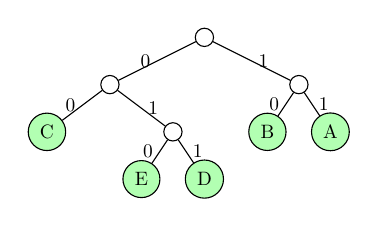
\begin{tikzpicture}[scale=0.4, every node/.style={scale=0.7}]
                    \node[draw, circle] (Root) at (5,5) {};
                    \node[draw, circle] (L) at (2,3.5) {};
                    \draw (Root) -- (L) node[midway, left] {0};
                    \node[draw, circle, fill=green!30] (C) at (0,2) {C};
                    \draw (L) -- (C) node[midway, left] {0};
                    \node[draw, circle] (LR) at (4,2) {};
                    \draw (L) -- (LR) node[midway, right] {1};
                    \node[draw, circle, fill=green!30] (E) at (3,0.5) {E};
                    \node[draw, circle, fill=green!30] (D) at (5,0.5) {D};
                    \draw (LR) -- (E) node[midway, left] {0};
                    \draw (LR) -- (D) node[midway, right] {1};
                    \node[draw, circle] (R) at (8,3.5) {};
                    \draw (Root) -- (R) node[midway, right] {1};
                    \node[draw, circle, fill=green!30] (B) at (7,2) {B};
                    \node[draw, circle, fill=green!30] (A) at (9,2) {A};
                    \draw (R) -- (B) node[midway, left] {0};
                    \draw (R) -- (A) node[midway, right] {1};
                \end{tikzpicture}
            \end{center}
        \end{column}
        \begin{column}{0.5\textwidth}
            \textbf{Decoding steps:}
            \begin{itemize}
                \item \textbf{10} $\rightarrow$ B
                \item \textbf{00} $\rightarrow$ C
                \item \textbf{011} $\rightarrow$ D
                \item \textbf{010} $\rightarrow$ E
            \end{itemize}
            
            \vspace{0.3cm}
            \textbf{Result:} BCDE
        \end{column}
    \end{columns}
    
    \vspace{0.3cm}
    \textit{Prefix-free property ensures unambiguous decoding!}
\end{frame}


%==============================================================================
\section{Practice Exercises}
%==============================================================================

\begin{frame}{Exercise 1: Build Huffman Code}
    \textbf{Problem:} Construct Huffman codes for the following source:
    
    \begin{center}
        \begin{tabular}{c|c}
            \toprule
            Symbol & Probability \\
            \midrule
            A & 0.40 \\
            B & 0.20 \\
            C & 0.15 \\
            D & 0.15 \\
            E & 0.10 \\
            \bottomrule
        \end{tabular}
    \end{center}
    
    \vspace{0.3cm}
    \textbf{Tasks:}
    \begin{enumerate}
        \item Build the Huffman tree step by step
        \item Assign codes to each symbol
        \item Calculate average code length
        \item Calculate entropy and efficiency
    \end{enumerate}
\end{frame}

\begin{frame}{Exercise 1: Solution --- Building the Tree}
    \textbf{Step-by-step merging:}
    
    \begin{enumerate}
        \item Initial: E(0.10), C(0.15), D(0.15), B(0.20), A(0.40)
        \item Merge E+C: [EC](0.25), D(0.15), B(0.20), A(0.40)
        \item Merge D+B: [EC](0.25), [DB](0.35), A(0.40)
        \item Merge [EC]+[DB]: [ECDB](0.60), A(0.40)
        \item Merge A+[ECDB]: Root(1.00)
    \end{enumerate}
    
    \begin{center}
        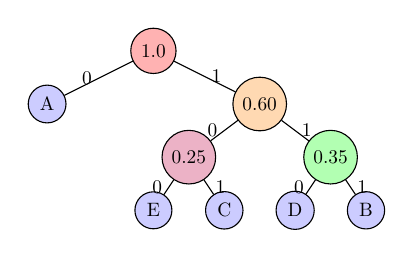
\begin{tikzpicture}[scale=0.45, every node/.style={scale=0.7}]
            \node[draw, circle, fill=red!30] (Root) at (5,5) {1.0};
            \node[draw, circle, fill=blue!20] (A) at (2,3.5) {A};
            \draw (Root) -- (A) node[midway, left] {0};
            \node[draw, circle, fill=orange!30] (ECDB) at (8,3.5) {0.60};
            \draw (Root) -- (ECDB) node[midway, right] {1};
            \node[draw, circle, fill=purple!30] (EC) at (6,2) {0.25};
            \node[draw, circle, fill=green!30] (DB) at (10,2) {0.35};
            \draw (ECDB) -- (EC) node[midway, left] {0};
            \draw (ECDB) -- (DB) node[midway, right] {1};
            \node[draw, circle, fill=blue!20] (E) at (5,0.5) {E};
            \node[draw, circle, fill=blue!20] (C) at (7,0.5) {C};
            \draw (EC) -- (E) node[midway, left] {0};
            \draw (EC) -- (C) node[midway, right] {1};
            \node[draw, circle, fill=blue!20] (D) at (9,0.5) {D};
            \node[draw, circle, fill=blue!20] (B) at (11,0.5) {B};
            \draw (DB) -- (D) node[midway, left] {0};
            \draw (DB) -- (B) node[midway, right] {1};
        \end{tikzpicture}
    \end{center}
\end{frame}

\begin{frame}{Exercise 1: Solution --- Final Codes}
    \textbf{Huffman Codes:}
    \begin{center}
        \begin{tabular}{c|c|c|c|c}
            \toprule
            Symbol & Probability & Code & Length & $p_i \times l_i$ \\
            \midrule
            A & 0.40 & 0 & 1 & 0.40 \\
            B & 0.20 & 111 & 3 & 0.60 \\
            C & 0.15 & 101 & 3 & 0.45 \\
            D & 0.15 & 110 & 3 & 0.45 \\
            E & 0.10 & 100 & 3 & 0.30 \\
            \midrule
            \multicolumn{4}{r|}{\textbf{Average Code Length:}} & \textbf{2.20} \\
            \bottomrule
        \end{tabular}
    \end{center}
    
    \vspace{0.3cm}
    \textbf{Entropy:} $H(X) = 2.122$ bits/symbol
    
    \textbf{Efficiency:} $\eta = \frac{2.122}{2.20} \times 100\% = \boxed{96.45\%}$
    
    \textbf{Redundancy:} $R = 2.20 - 2.122 = \boxed{0.078 \text{ bits/symbol}}$
\end{frame}

\begin{frame}{Exercise 2: Text Compression}
    \textbf{Problem:} Analyze and compress the following text using Huffman coding:
    
    \begin{block}{Text (30 characters)}
        \texttt{ABRACADABRA\_ABRACADABRA\_ABRA}
    \end{block}
    
    \vspace{0.3cm}
    \textbf{Tasks:}
    \begin{enumerate}
        \item Count frequency of each character
        \item Calculate probabilities
        \item Build Huffman tree
        \item Calculate compression ratio vs 8-bit ASCII
    \end{enumerate}
    
    \vspace{0.3cm}
    \textit{Hint: Count carefully --- A appears very frequently!}
\end{frame}

\begin{frame}{Exercise 2: Solution}
    \textbf{Character Analysis:}
    \begin{center}
        \begin{tabular}{c|c|c}
            \toprule
            Char & Count & Probability \\
            \midrule
            A & 12 & 0.40 \\
            B & 6 & 0.20 \\
            R & 6 & 0.20 \\
            \_ & 2 & 0.067 \\
            C & 2 & 0.067 \\
            D & 2 & 0.067 \\
            \midrule
            Total & 30 & 1.00 \\
            \bottomrule
        \end{tabular}
    \end{center}
    
    \textbf{Huffman Codes:} A=0, B=10, R=110, \_=1110, C=11110, D=11111
    
    \textbf{Average length:} $L_{avg} = 2.27$ bits/char
    
    \textbf{Compression:} $\frac{2.27}{8} = 28.4\%$ of original size!
\end{frame}

\begin{frame}{Exercise 3: Image Pixel Encoding}
    \textbf{Problem:} A grayscale image has the following pixel value distribution:
    
    \begin{center}
        \begin{tabular}{c|c}
            \toprule
            Pixel Value & Probability \\
            \midrule
            0 (Black) & 0.05 \\
            85 (Dark Gray) & 0.15 \\
            170 (Light Gray) & 0.35 \\
            255 (White) & 0.45 \\
            \bottomrule
        \end{tabular}
    \end{center}
    
    \textbf{Tasks:}
    \begin{enumerate}
        \item Build Huffman codes for pixel values
        \item Calculate average bits per pixel
        \item Compare with fixed 8-bit encoding
        \item Calculate compression ratio
    \end{enumerate}
\end{frame}

\begin{frame}{Exercise 3: Solution}
    \textbf{Huffman Tree Construction:}
    \begin{enumerate}
        \item Merge 0(0.05) + 85(0.15) = [0,85](0.20)
        \item Merge [0,85](0.20) + 170(0.35) = [0,85,170](0.55)
        \item Merge 255(0.45) + [0,85,170](0.55) = Root(1.00)
    \end{enumerate}
    
    \begin{center}
        \begin{tabular}{c|c|c|c}
            \toprule
            Pixel & Prob & Code & Length \\
            \midrule
            255 (White) & 0.45 & 0 & 1 \\
            170 (Light Gray) & 0.35 & 10 & 2 \\
            85 (Dark Gray) & 0.15 & 110 & 3 \\
            0 (Black) & 0.05 & 111 & 3 \\
            \bottomrule
        \end{tabular}
    \end{center}
    
    $L_{avg} = 0.45(1) + 0.35(2) + 0.15(3) + 0.05(3) = \boxed{1.75 \text{ bits/pixel}}$
    
    \textbf{Compression:} $\frac{1.75}{8} = 21.9\%$ --- \textbf{78\% space saved!}
\end{frame}

%==============================================================================
\section{Real-World Applications}
%==============================================================================

\begin{frame}{Huffman Coding in JPEG}
    \textbf{How JPEG Uses Huffman Coding:}
    
    \begin{columns}
        \begin{column}{0.5\textwidth}
            \textbf{JPEG Pipeline:}
            \begin{enumerate}
                \item Color space conversion (RGB $\rightarrow$ YCbCr)
                \item Block splitting (8$\times$8 pixels)
                \item DCT (Discrete Cosine Transform)
                \item Quantization
                \item \textcolor{red}{\textbf{Huffman Coding}}
            \end{enumerate}
            
            \vspace{0.3cm}
            \textbf{Why Huffman here?}
            \begin{itemize}
                \item After DCT, many coefficients are 0
                \item Small values are common
                \item Perfect for variable-length coding!
            \end{itemize}
        \end{column}
        \begin{column}{0.5\textwidth}
            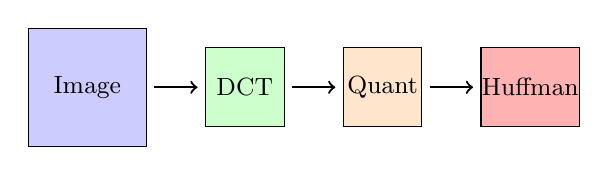
\begin{tikzpicture}[scale=0.5]
                \draw[fill=blue!20] (0,0) rectangle (3,3);
                \node at (1.5,1.5) {\small Image};
                \draw[->,thick] (3.2,1.5) -- (4.3,1.5);
                \draw[fill=green!20] (4.5,0.5) rectangle (6.5,2.5);
                \node at (5.5,1.5) {\small DCT};
                \draw[->,thick] (6.7,1.5) -- (7.8,1.5);
                \draw[fill=orange!20] (8,0.5) rectangle (10,2.5);
                \node at (9,1.5) {\small Quant};
                \draw[->,thick] (10.2,1.5) -- (11.3,1.5);
                \draw[fill=red!30] (11.5,0.5) rectangle (14,2.5);
                \node at (12.75,1.5) {\small Huffman};
            \end{tikzpicture}
            
            \vspace{0.5cm}
            \textbf{Result:}
            \begin{itemize}
                \item 10 MB photo $\rightarrow$ 500 KB
                \item 95\% compression!
            \end{itemize}
        \end{column}
    \end{columns}
\end{frame}

\begin{frame}{Huffman in ZIP and DEFLATE}
    \textbf{DEFLATE Algorithm (used in ZIP, gzip, PNG):}
    
    \begin{block}{Two-Stage Compression}
        \begin{enumerate}
            \item \textbf{LZ77:} Find repeated patterns, replace with references
            \item \textbf{Huffman:} Encode the LZ77 output efficiently
        \end{enumerate}
    \end{block}
    
    \vspace{0.3cm}
    \begin{columns}
        \begin{column}{0.5\textwidth}
            \textbf{Example:}
            
            Original: ``ABCABCABC''
            
            After LZ77: ``ABC[back 3, len 6]''
            
            After Huffman: Even shorter!
        \end{column}
        \begin{column}{0.5\textwidth}
            \textbf{Used in:}
            \begin{itemize}
                \item ZIP files
                \item gzip compression
                \item PNG images
                \item HTTP compression
                \item PDF files
            \end{itemize}
        \end{column}
    \end{columns}
\end{frame}

\begin{frame}{Huffman in MP3 Audio}
    \textbf{MP3 Compression Pipeline:}
    
    \begin{enumerate}
        \item \textbf{Psychoacoustic Model:} Remove sounds humans can't hear
        \item \textbf{MDCT:} Transform to frequency domain
        \item \textbf{Quantization:} Reduce precision
        \item \textbf{Huffman Coding:} Compress the quantized values
    \end{enumerate}
    
    \vspace{0.3cm}
    \begin{alertblock}{Why Huffman Works Well for Audio}
        \begin{itemize}
            \item After quantization, small values dominate
            \item Zero is the most common value
            \item Huffman gives short codes to common values
            \item Result: 10:1 compression with good quality!
        \end{itemize}
    \end{alertblock}
    
    \vspace{0.2cm}
    \textbf{CD Quality:} 1411 kbps $\rightarrow$ \textbf{MP3:} 128-320 kbps
\end{frame}

%==============================================================================
\section{Variants and Extensions}
%==============================================================================

\begin{frame}{Adaptive Huffman Coding}
    \textbf{Problem with Static Huffman:}
    \begin{itemize}
        \item Need to know all probabilities beforehand
        \item Must send code table with compressed data
        \item Two passes over data required
    \end{itemize}
    
    \vspace{0.3cm}
    \begin{block}{Adaptive (Dynamic) Huffman}
        \begin{itemize}
            \item Build tree as you encode/decode
            \item Update tree after each symbol
            \item No need to transmit code table!
            \item Single pass over data
        \end{itemize}
    \end{block}
    
    \vspace{0.3cm}
    \textbf{Algorithms:}
    \begin{itemize}
        \item FGK Algorithm (Faller, Gallager, Knuth)
        \item Vitter's Algorithm (more efficient)
    \end{itemize}
\end{frame}

\begin{frame}{Canonical Huffman Codes}
    \textbf{Problem:} Different Huffman trees can have same code lengths
    
    \begin{block}{Canonical Huffman}
        Standardized way to assign codes given code lengths:
        \begin{enumerate}
            \item Sort symbols by code length, then alphabetically
            \item First code of length $L$ is 0...0 ($L$ zeros)
            \item Next code = previous code + 1
            \item When length increases, shift left and add 0
        \end{enumerate}
    \end{block}
    
    \vspace{0.3cm}
    \textbf{Advantages:}
    \begin{itemize}
        \item Only need to store code lengths (not full tree)
        \item Faster decoding with lookup tables
        \item Used in DEFLATE, JPEG, and many formats
    \end{itemize}
\end{frame}

\begin{frame}{Beyond Huffman: Modern Alternatives}
    \begin{columns}
        \begin{column}{0.5\textwidth}
            \textbf{Arithmetic Coding:}
            \begin{itemize}
                \item Encodes entire message as one number
                \item Can achieve fractional bits per symbol
                \item Closer to entropy than Huffman
                \item Used in JPEG 2000, H.264
            \end{itemize}
            
            \vspace{0.3cm}
            \textbf{ANS (Asymmetric Numeral Systems):}
            \begin{itemize}
                \item Modern alternative (2009)
                \item Speed of Huffman
                \item Compression of arithmetic coding
                \item Used in Zstandard, LZFSE
            \end{itemize}
        \end{column}
        \begin{column}{0.5\textwidth}
            \textbf{Comparison:}
            \begin{center}
                \begin{tabular}{l|c|c}
                    \toprule
                    Method & Speed & Compression \\
                    \midrule
                    Huffman & Fast & Good \\
                    Arithmetic & Slow & Best \\
                    ANS & Fast & Best \\
                    \bottomrule
                \end{tabular}
            \end{center}
            
            \vspace{0.5cm}
            \begin{alertblock}{Huffman Still Relevant!}
                Simple, fast, patent-free, and ``good enough'' for many applications.
            \end{alertblock}
        \end{column}
    \end{columns}
\end{frame}

%==============================================================================
\section{Summary}
%==============================================================================

\begin{frame}{Key Takeaways}
    \begin{enumerate}
        \item \textbf{Huffman coding} builds optimal prefix-free codes \textbf{bottom-up}
        
        \item \textbf{Algorithm:} Repeatedly merge two lowest-probability nodes
        
        \item \textbf{Optimality:} Guaranteed minimum average code length
        \begin{equation*}
            H(X) \leq L_{avg} < H(X) + 1
        \end{equation*}
        
        \item \textbf{vs Shannon-Fano:} Same or better, never worse
        
        \item \textbf{Applications:} JPEG, MP3, ZIP, PNG, and more
        
        \item \textbf{Variants:} Adaptive, Canonical, Extended Huffman
    \end{enumerate}
    
    \vspace{0.3cm}
    \begin{block}{Remember}
        Huffman = Greedy + Bottom-up = Optimal!
    \end{block}
\end{frame}

\begin{frame}{Important Formulas Summary}
    \begin{block}{Entropy}
        $H(X) = -\sum_{i=1}^{n} p_i \log_2 p_i$
    \end{block}
    
    \begin{block}{Average Code Length}
        $L_{avg} = \sum_{i=1}^{n} p_i \cdot l_i$
    \end{block}
    
    \begin{block}{Efficiency}
        $\eta = \frac{H(X)}{L_{avg}} \times 100\%$
    \end{block}
    
    \begin{block}{Redundancy}
        $R = L_{avg} - H(X)$
    \end{block}
    
    \begin{block}{Compression Ratio}
        $CR = \frac{\text{Original Size}}{\text{Compressed Size}}$
    \end{block}
\end{frame}

\begin{frame}{Practice Problems}
    \textbf{Problem 1:} Build Huffman codes for: P(A)=0.30, P(B)=0.25, P(C)=0.20, P(D)=0.15, P(E)=0.10
    
    \vspace{0.3cm}
    \textbf{Problem 2:} A file has 1000 characters with frequencies:
    \begin{center}
        \begin{tabular}{c|ccccc}
            Char & a & b & c & d & e \\
            Count & 450 & 250 & 150 & 100 & 50 \\
        \end{tabular}
    \end{center}
    Calculate compression ratio vs 8-bit ASCII.
    
    \vspace{0.3cm}
    \textbf{Problem 3:} Decode ``0110100111'' using codes: A=0, B=10, C=110, D=111
    
    \vspace{0.3cm}
    \textbf{Problem 4:} Compare Huffman and Shannon-Fano for: 0.4, 0.2, 0.2, 0.1, 0.1
\end{frame}

\begin{frame}
    \begin{center}
        \Huge{\textbf{Thank You!}}
        
        \vspace{1cm}
        \Large{Questions?}
        
        \vspace{1.5cm}
        \normalsize
        \textit{``I was able to do this because I didn't know it was supposed to be hard.''}
        
        \vspace{0.3cm}
        --- David Huffman
    \end{center}
\end{frame}

\end{document}
